\documentclass{sigchi}

% Use this command to override the default ACM copyright statement (e.g. for preprints). 
% Consult the conference website for the camera-ready copyright statement.


%% EXAMPLE BEGIN -- HOW TO OVERRIDE THE DEFAULT COPYRIGHT STRIP -- (July 22, 2013 - Paul Baumann)
% \toappear{Permission to make digital or hard copies of all or part of this work for personal or classroom use is 	granted without fee provided that copies are not made or distributed for profit or commercial advantage and that copies bear this notice and the full citation on the first page. Copyrights for components of this work owned by others than ACM must be honored. Abstracting with credit is permitted. To copy otherwise, or republish, to post on servers or to redistribute to lists, requires prior specific permission and/or a fee. Request permissions from permissions@acm.org. \\
% {\emph{CHI'14}}, April 26--May 1, 2014, Toronto, Canada. \\
% Copyright \copyright~2014 ACM ISBN/14/04...\$15.00. \\
% DOI string from ACM form confirmation}
%% EXAMPLE END -- HOW TO OVERRIDE THE DEFAULT COPYRIGHT STRIP -- (July 22, 2013 - Paul Baumann)


% Arabic page numbers for submission. 
% Remove this line to eliminate page numbers for the camera ready copy
% \pagenumbering{arabic}


% Load basic packages
\usepackage{balance}  % to better equalize the last page
\usepackage{graphics} % for EPS, load graphicx instead
\usepackage{times}    % comment if you want LaTeX's default font
\usepackage{url}      % llt: nicely formatted URLs

% llt: Define a global style for URLs, rather that the default one
\makeatletter
\def\url@leostyle{%
  \@ifundefined{selectfont}{\def\UrlFont{\sf}}{\def\UrlFont{\small\bf\ttfamily}}}
\makeatother
\urlstyle{leo}


% To make various LaTeX processors do the right thing with page size.
\def\pprw{8.5in}
\def\pprh{11in}
\special{papersize=\pprw,\pprh}
\setlength{\paperwidth}{\pprw}
\setlength{\paperheight}{\pprh}
\setlength{\pdfpagewidth}{\pprw}
\setlength{\pdfpageheight}{\pprh}

% Make sure hyperref comes last of your loaded packages, 
% to give it a fighting chance of not being over-written, 
% since its job is to redefine many LaTeX commands.
\usepackage[pdftex]{hyperref}
\hypersetup{
pdftitle={SIGCHI Conference Proceedings Format},
pdfauthor={LaTeX},
pdfkeywords={SIGCHI, proceedings, archival format},
bookmarksnumbered,
pdfstartview={FitH},
colorlinks,
citecolor=black,
filecolor=black,
linkcolor=black,
urlcolor=black,
breaklinks=true,
}

% create a shortcut to typeset table headings
\newcommand\tabhead[1]{\small\textbf{#1}}


% End of preamble. Here it comes the document.
\begin{document}

\title{User-Defined Game Control with \\Smart Glasses in Public Space}

\numberofauthors{6}
\author{
  \alignauthor 1st Author Name\\
    \affaddr{Affiliation}\\
    \affaddr{Address}\\
    \email{e-mail address}\\
    \affaddr{Optional phone number}
  \alignauthor 2nd Author Name\\
    \affaddr{Affiliation}\\
    \affaddr{Address}\\
    \email{e-mail address}\\
    \affaddr{Optional phone number}    
  \alignauthor 3rd Author Name\\
    \affaddr{Affiliation}\\
    \affaddr{Address}\\
    \email{e-mail address}\\
    \affaddr{Optional phone number}
  \alignauthor 4rd Author Name\\
    \affaddr{Affiliation}\\
    \affaddr{Address}\\
    \email{e-mail address}\\
    \affaddr{Optional phone number}
  \alignauthor 5rd Author Name\\
    \affaddr{Affiliation}\\
    \affaddr{Address}\\
    \email{e-mail address}\\
    \affaddr{Optional phone number}
  \alignauthor 6rd Author Name\\
    \affaddr{Affiliation}\\
    \affaddr{Address}\\
    \email{e-mail address}\\
    \affaddr{Optional phone number}
}

\maketitle

\begin{abstract}
Without specific game controller and direct-touch, game control on Smart Glasses differs with existing console and mobile games. Although current game control set on Smart Glasses is explored by developers based on system limitation, the set is not reflective of user behavior.
To create better game control, we presented an user-defined game control study in public space to collect user behavior. In all, 2448 game controls from 24 participants were logged, analyzed, and paired with think-aloud data for 17 commands performed with 3 interaction methods (On-Body, In-Air and Phone) and 2 glasses forms (Google Glass and Epson BT-100). 
Our findings indicate that users choose area relatively unobtrusive to perform the game control, and glasses form does influence how users creates game control. We also present a complete user-defined game control set with agreement scores and taxonomy. 
Our results will help designers create better game control sets informed by user behavior.
\end{abstract}

\keywords{
	Guides; instructions; author's kit; conference publications;
	keywords should be separated by a semi-colon. \newline
	\textcolor{red}{Optional section to be included in your final version, 
  but strongly encouraged.}
}

\category{H.5.m.}{Information Interfaces and Presentation (e.g. HCI)}{Miscellaneous}

See: \url{http://www.acm.org/about/class/1998/}
for more information and the full list of ACM classifiers
and descriptors. \newline
\textcolor{red}{Optional section to be included in your final version, 
but strongly encouraged. On the submission page only the classifiers’ 
letter-number combination will need to be entered.}

\section{Introduction}

%A. Review現有遊戲平台及操作方式。
%B. Smart Glass帶來新的可能性,跟傳統遊戲的區別。 
%C. 現有的Smart Glass Gaming有哪些,而且目前體驗很差。
%D. 我們認為造成體驗差的原因,跟我們的解法。


\section{Related Work}

    \subsection{Game Control}

    \subsection{Glass Input}

    \subsection{Gaming in Public Space}

    \subsection{User-Defined Gesture}

\section{Developing a User-Defined Game Control Set}
%需要描述場域嘛?


    \subsection {Overview and Rationale}

    \subsection {Game Task Set}

    Casual game is one of the game categories with most players\cite{esa_ef_2014}, it is shown high potential in public gaming\cite{Jurgelionis:2011:PET:2027456.2027462,Reis:2012:EMC:2405577.2405651,Biskupski:2014:DEB:2559206.2580097}. We choose top 90 casual games\cite{TopGames} from existing platforms, including PC,console and mobile games (30 games for each) by crawling and analyzing the sale and download count data from famous gaming websites\cite{appannie,VGChartz,Steam,GameStop}. We invited 3 experienced game developer to review these top 90 casual games. They find out totally 26 game tasks, and removed 9 tasks which only be used once in specific games. At last, we get a general casual game task set with 17 tasks, which can completely support 90\% of our top casual games. We describe our general casual game task set in Table \ref{tab:table1}.

  \begin{table}
    \centering
    \begin{tabular}{|c|l|l|}
      \hline
      \tabhead{\#} &
      \multicolumn{1}{|p{0.4\columnwidth}|}{\centering\tabhead{Description}} &
      \multicolumn{1}{|p{0.4\columnwidth}|}{\centering\tabhead{Used in Famous Game}} \\
      \hline
      1 & Single select & Clash of Clans, Plague Inc.\\
      \hline
      2 & Vertical menu & Puzzle\&Dragon, PeggleHD \\
      \hline
      3 & Horizontal menu & Clash of Clans, PeggleHD\\
      \hline
      4 & Move left and right & Temple Run, Super Mario\\
      \hline
      5 & Move in 4 directions & 1943, RaidenX\\
      \hline
      6 & Switch 2 objects & Candy Crush, Bejeweled\\
      \hline
      7 & Move object to position & World of Goo, The Sim\\
      \hline
      8 & Draw a path & Draw Something, P\&D\\
      \hline
      9 & Throw an object (in-2D) & Angry Birds, PeggleHD\\
      \hline
      10 & Note highway & RockSmith, Deemo\\
      \hline
      11 & Rotate an object (Z-axis) & Zuma, PeggleHD \\
      \hline
      12 & Rotate an object (Y-axis) & Spore, The Sim\\
      \hline
      13 & Avatar jump & Temple Run, Super Mario\\
      \hline
      14 & Avatar 3D move & Spore, Tintin\\
      \hline
      15 & Avatar attack & Minecraft, Terraria\\
      \hline
      16 & Avatar squat & Temple Run, Minecraft\\
      \hline
      17 & 3D Viewport control & The Sim, Spore\\
      \hline

    \end{tabular}
    \caption{Summary of our general casual game task set. We named several famous games which uses these tasks.}
    \label{tab:table1}
  \end{table}


  \subsection {Participants}
  We recruited twenty-four participants from the general public for our study. Twelve were female. Average age was 23.2 (\textsl{sd} = 2.72). All participants are right-handed and none of them had used a Smart Glasses. About their gaming experience, according to our investigation, most participants play games at least one time per week (see Figure~\ref{fig:figureFrequency}). It takes 1.36 hours (\textsl{sd} = 0.89) for participants to play games a time. Moreover, 58\% of them indicated that their main gaming platforms were on mobile phones, 38\% were on PCs, and only 4\% were on consoles. Another important factor of gaming experience is the familiarity of game controllers. The result showed that, compared with joysticks, most of them were more familiar with keyboards, mouses and touch screens (see Figure~\ref{fig:figureFamiliarity}).
  %\begin{figure}[!h]
  %\centering
  %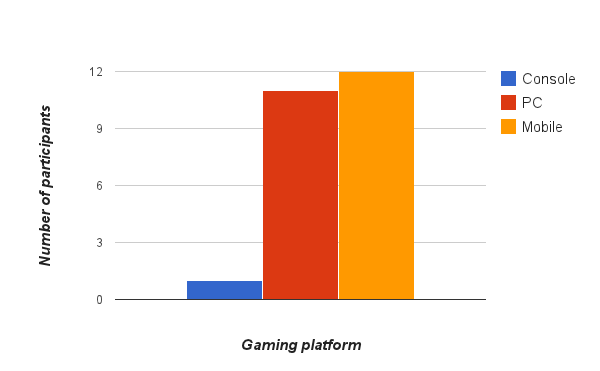
\includegraphics[width=0.9\columnwidth]{Platform}
  %\caption{With Caption Below, be sure to have a good resolution image
  %  (see item D within the preparation instructions).}
  %\label{fig:figurePlatform}
  %\end{figure} 
  \begin{figure}[!h]
  \centering
  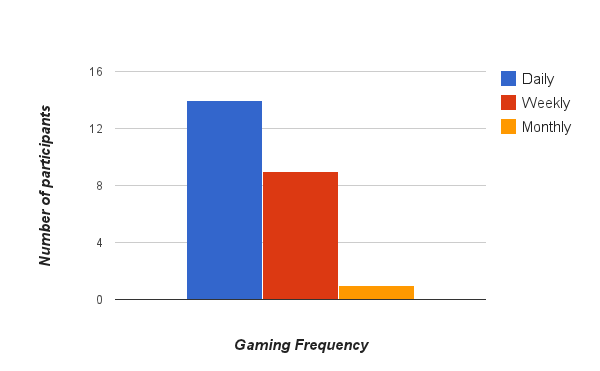
\includegraphics[width=0.9\columnwidth]{Frequency}
  \caption{With Caption Below, be sure to have a good resolution image
    (see item D within the preparation instructions).}
  \label{fig:figureFrequency}
  \end{figure}
  \begin{figure}[!h]
  \centering
  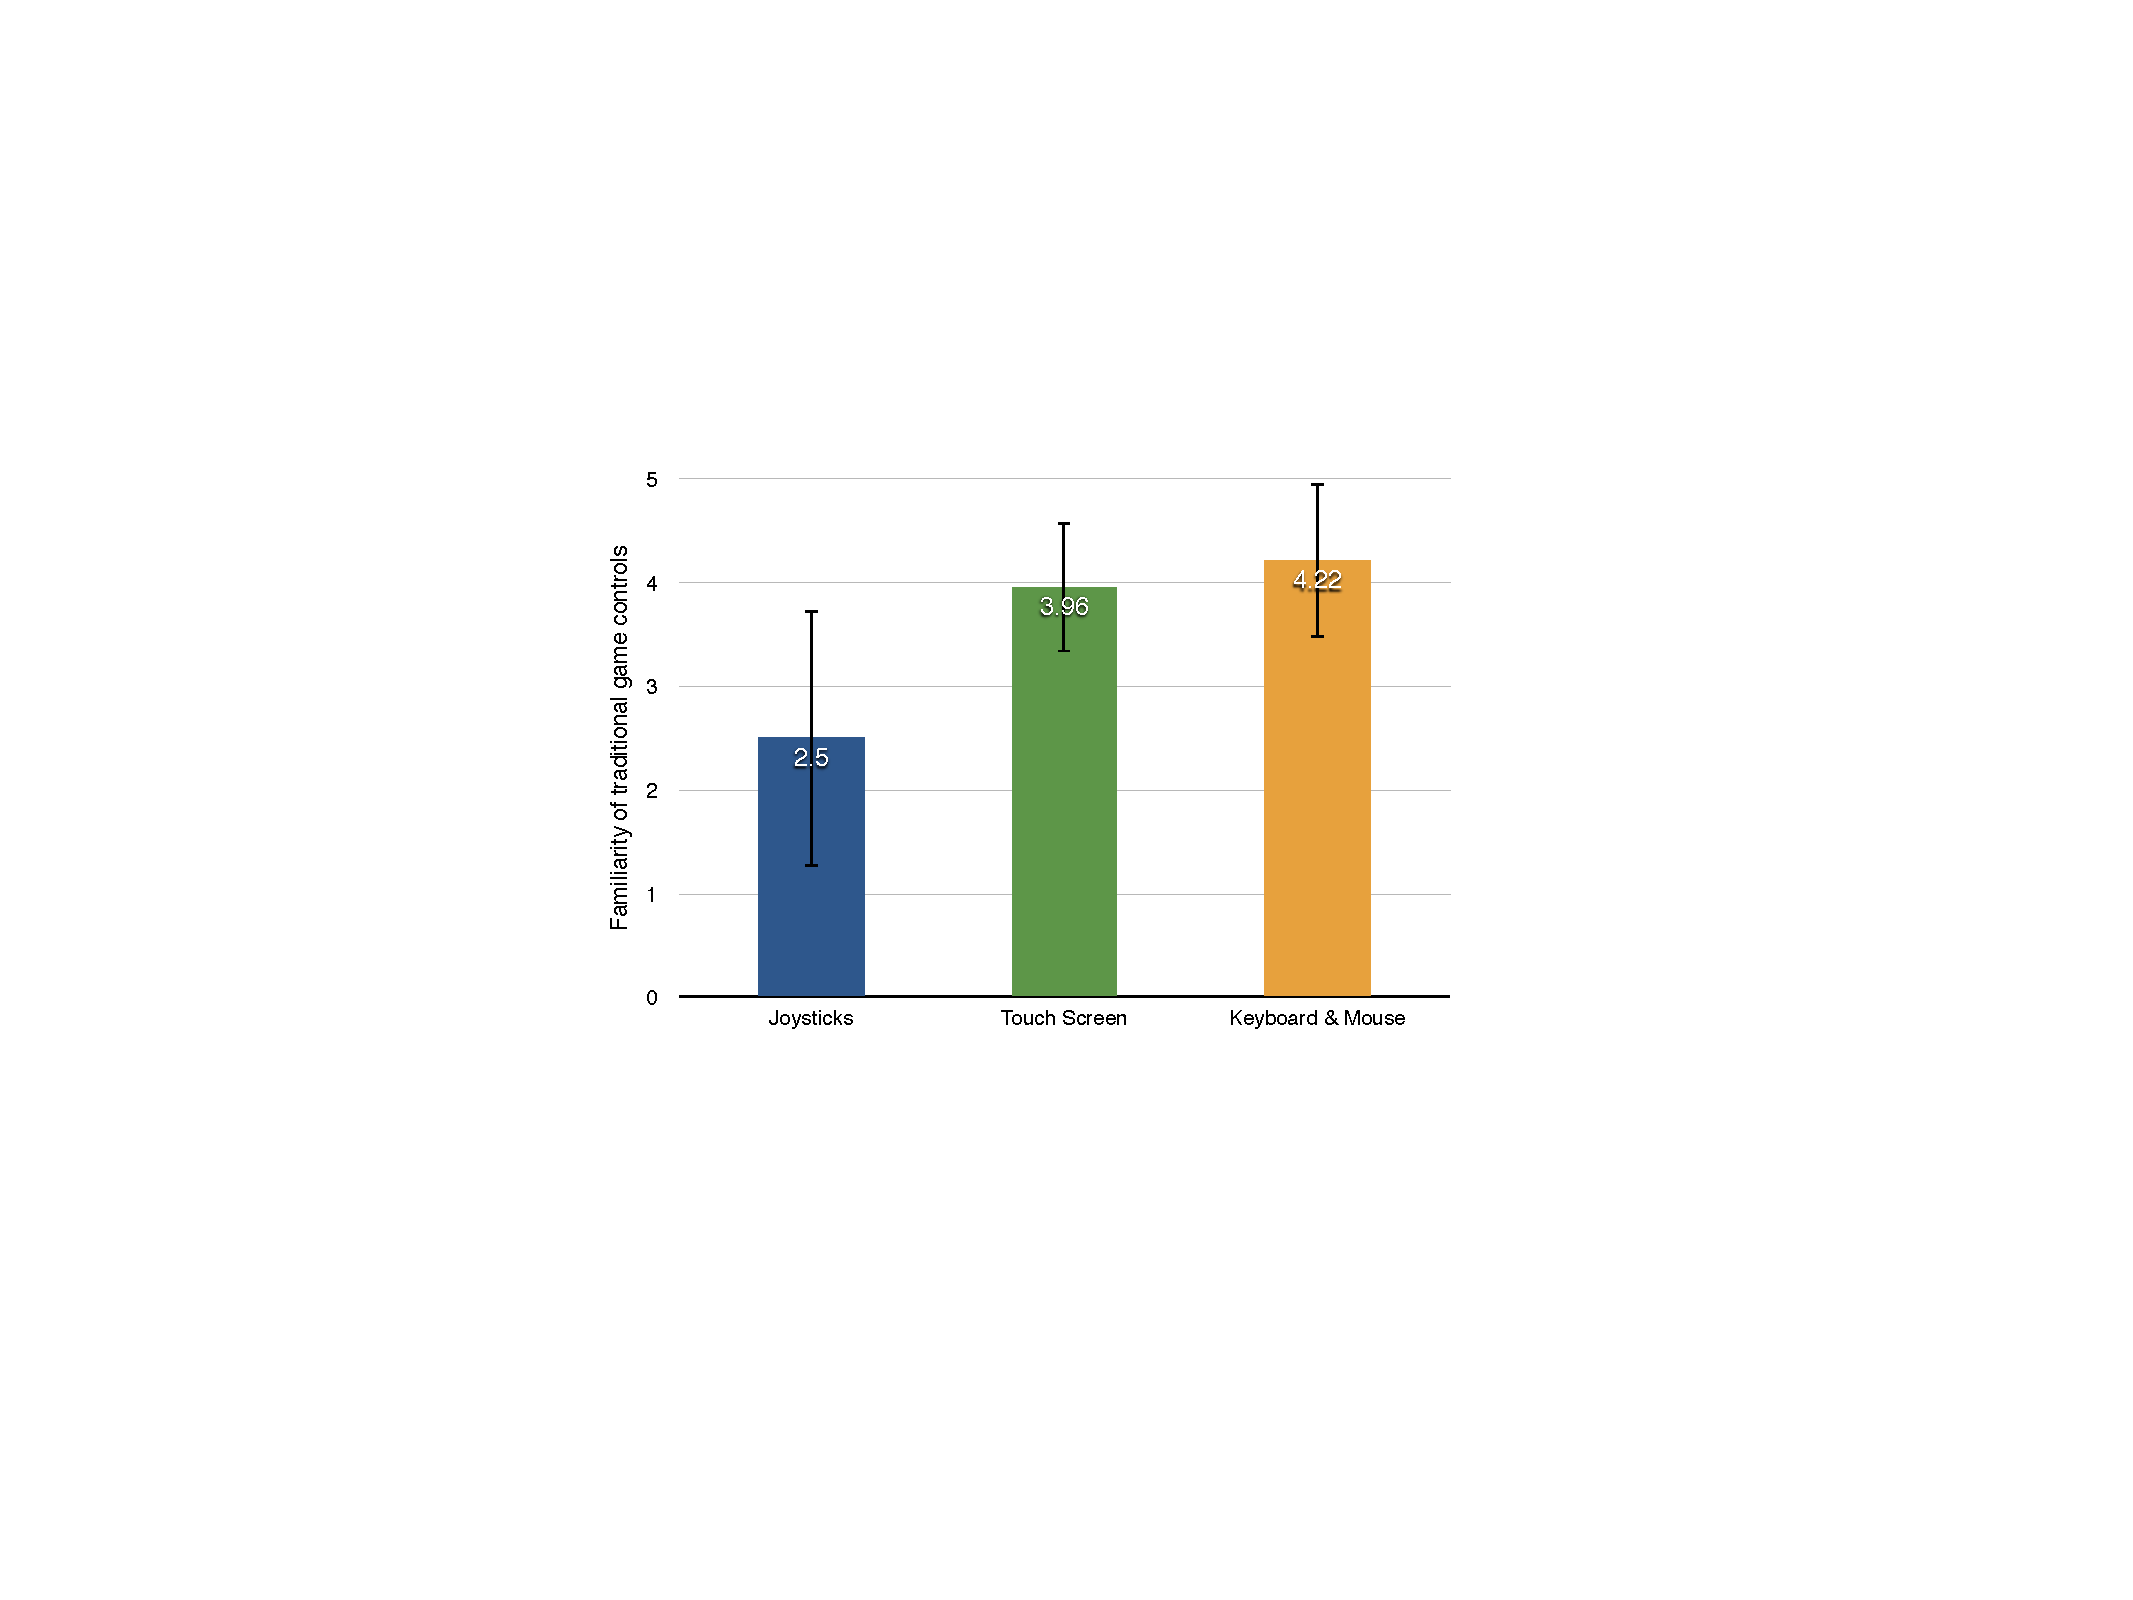
\includegraphics[width=0.9\columnwidth]{Familiarity}
  \caption{With Caption Below, be sure to have a good resolution image
    (see item D within the preparation instructions).}
  \label{fig:figureFamiliarity}
  \end{figure}   

  \subsection {Glass Forms}
  There are many Smart Glasses with different screen sizes and screen placement on the current market. To observe the effect of different display designs upon the study result, our study conducted on two famous Smart Glasses, Epson and Google Glass. The display of Epson BT-100 is located in front of the user's eyes with $960 \times 540$ resolution (equivalent of a 320" screen from 20 m away). And Google Glass locates its display above the user's right eye with $640 \times 360$ resolution (equivalent of a 25" screen from 2.4 m away).       

    \subsection {Interaction Methods}

    \subsection {Procedure}

\section{Results}

Our results include game control taxonomies, the user-defined gesture sets, user rating, subjective responses, and qualitative observations for each interaction methods.

  \subsection{Preference Between Interaction Methods}

  \subsection{Behavior with Different Glasses Forms}

  \subsection{Classification of Game Controls}
  %Taxonomy的圖放在這邊
  %Kappa Value也要在這邊交代

  \subsection{User-Defined Game Control Sets}
   \subsubsection{Agreement}
   \subsubsection{Conflict and Coverage}
   \subsubsection{Properties of the User-defined Gesture Sets}
   \subsubsection{Taxonometric Breakdown of User-defined Game Controls}

  \subsection{Mental Model Observations}
    \subsubsection{Social Acceptance and Control Area}
    \subsubsection{Metaphor from Exisiting Game Control}

  \section{Discussion}
    \subsubsection{Users' and Designers' Gestures}
    \subsubsection{Implications for In-Air Gesture Technology}
    \subsubsection{Implications for On-Body Input Technology}
    \subsubsection{Implications for User Interfaces}
    \subsubsection{Limitation and Next Steps}
    %Glass Forms 只有兩種
    %Culture問題?
    %Interaction with 桌椅?


\section{Conclusion}


%It is important that you write for the SIGCHI audience.  Please read
%previous years' Proceedings to understand the writing style and
%conventions that successful authors have used.  It is particularly
%important that you state clearly what you have done, not merely what
%you plan to do, and explain how your work is different from previously
%published work, i.e., what is the unique contribution that your work
%makes to the field?  Please consider what the reader will learn from
%your submission, and how they will find your work useful.  If you
%write with these questions in mind, your work is more likely to be
%successful, both in being accepted into the Conference, and in
%influencing the work of our field.

\section{Acknowledgments}

%We thank CHI, PDC and CSCW volunteers, and all publications support
%and staff, who wrote and provided helpful comments on previous
%versions of this document.  Some of the references cited in this paper
%are included for illustrative purposes only.  \textbf{Don't forget
%to acknowledge funding sources as well}, so you don't wind up
%having to correct it later.

% Balancing columns in a ref list is a bit of a pain because you
% either use a hack like flushend or balance, or manually insert
% a column break.  http://www.tex.ac.uk/cgi-bin/texfaq2html?label=balance
% multicols doesn't work because we're already in two-column mode,
% and flushend isn't awesome, so I choose balance.  See this
% for more info: http://cs.brown.edu/system/software/latex/doc/balance.pdf
%
% Note that in a perfect world balance wants to be in the first
% column of the last page.
%
% If balance doesn't work for you, you can remove that and
% hard-code a column break into the bbl file right before you
% submit:
%
% http://stackoverflow.com/questions/2149854/how-to-manually-equalize-columns-
% in-an-ieee-paper-if-using-bibtex
%
% Or, just remove \balance and give up on balancing the last page.
%
\balance

%\section{References format}
%References must be the same font size as other body text.
% REFERENCES FORMAT
% References must be the same font size as other body text.

\bibliographystyle{acm-sigchi}
\bibliography{sample}
\end{document}
